\icode{N24J-MI-SI-L3-261108-001}
\nceeID[4]{2024河北}{5}
如图，弹簧测力计下端挂有质量为\qty{0.20}{kg}的光滑均匀球体，球体静止于带有固定档板的斜面上，斜面倾角为\qty{30}{\degree}，档板与斜面的夹角为\qty{60}{\degree}。若弹簧测力计位于竖直方向，读数为\qty{1.0}{N}，\(g\)取\qty{10}{m/s^2}，档板对球体支持力大小为\paren[]

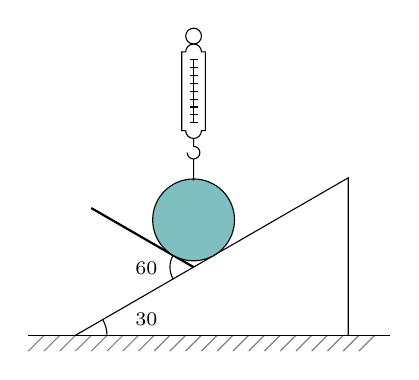
\begin{tikzpicture}[font=\scriptsize]
    \draw (0,0)--(30:4)--++(-90:2);
	\draw[thick] (30:{sqrt(3)})--++(150:1.5);
	\draw (30:{sqrt(3)-.3}) arc(-150:-210:.3) (.4,0) arc(0:30:.4);
	\draw[fill=teal!50] (1.5,{.5*sqrt(3)+.6}) circle({.3*sqrt(3)});
	\draw (1.4,2.6) arc(-180:0:.1)--(1.65,2.6)--(1.65,3.6)--(1.6,3.6) arc(0:180:.1)--(1.35,3.6)--(1.35,2.6)--(1.4,2.6) (1.5,2.5)--(1.5,2.4) arc(90:-180:.08) (1.5,2.24)--(1.5,{.5*sqrt(3)+1.1});
	\draw (1.5,3.8) circle(.1);
	\foreach \y in {2.7,2.8,...,3.5}
		\draw[thin] (1.45,\y)--++(.1,0);
	\draw (1.5,2.7)--(1.5,3.5) (1.45,2.7)--(1.55,2.7) (1.45,3.5)--(1.55,3.5);
	\foreach \x in {-.6,-.4,...,3.8}
		\draw[gray] (\x,-.2)--++(.2,.2);
	\draw (-.6,0)--(4,0);
	\node at(.9,.2){\qty{30}{\degree}};
	\node at(.9,.85){\qty{60}{\degree}};
\end{tikzpicture}
\begin{choices}
	\item\(\frac{\sqrt{3}}{3}\)\,\qty{}{N}
	\item \qty{1.0}{N}
	\item\(\frac{2\sqrt{3}}{3}\)\,\qty{}{N}
	\item \qty{2.0}{N}
\end{choices}
\begin{answer}
	A\qquad 提示：分解力，合成力。
\end{answer}